\documentclass[grad,numbers]{coppe}
\usepackage{amsmath,amssymb}
\usepackage{hyperref}
\usepackage[utf8]{inputenc}
\usepackage[brazil]{babel}
\usepackage[T1]{fontenc}
\usepackage{graphicx}

\makelosymbols
\makeloabbreviations

\begin{document}
  \title{Análise de Notícias do Mercado Financeiro Utilizando Processamento de Linguagem Natural e Aprendizado de Máquina Para Decisões de Swing Trade}
  \foreigntitle{Financial Market News Analysis Using Natural Language Processing and Machine Learning for Swing Trade Decisions}
  \author{Lucas}{Gama Canto}
  \advisor{Prof.}{Heraldo Luís}{Silveira de Almeida}{D.Sc.}

  \examiner{Prof.}{[TODO]Nome do Primeiro Examinador Sobrenome}{D.Sc.}
  \examiner{Prof.}{[TODO]Nome do Segundo Examinador Sobrenome}{Ph.D.}
  \examiner{Prof.}{[TODO]Nome do Terceiro Examinador Sobrenome}{D.Sc.}
  
  \department{ECA}
  
  \date{03}{2020}

  \keyword{Aprendizado de Máquina}
  \keyword{Processamento de Linguagem Natural}
  \keyword{Mercado Financeiro}

  \maketitle

  \frontmatter
  
  \makecatalog
  
  \dedication{Ao povo brasileiro, pela total contribuição em minha graduação.}

  \chapter*{Agradecimentos}

	  \paragraph{}Gostaria de agradecer a todas as pessoas e situações que tornaram este momento possível. Em especial, meus pais Benedita e Manoel, pelo suporte e esforço incondicional em apoiar minha decisão de vir estudar engenharia no Rio de Janeiro, aos professores da graduação, que me fizeram evoluir no âmbito acadêmico, profissional e pessoal, em especial ao meu orientador e professor Heraldo, que não mediu esforços para me ajudar neste trabalho, e aos amigos que me apoiaram e participaram do meu processo de graduação.

  \begin{abstract}

	  \paragraph{}Com o objetivo de automatizar análises fundamentalistas de mercado, o uso de tecnologia para processamento de texto vem sendo utilizado constantemente no meio acadêmico\cite{nlp-academics} e profissional\cite{nlp-industry}. De forma a contribuir para este campo em crescimento, este trabalho discorre um estudo acerca da criação de modelos preditivos sobre a valorização ou desvalorização de ações na bolsa de valores do Brasil (B3, antiga Bovespa) a partir de notícias sobre o mercado brasileiro de forma a auxiliar decisões de Swing Trade, ou seja, compra e venda de ações dentro de uma janela de tempo maior que um dia.
	  \paragraph{}Para isto, o presente projeto utiliza o framework PyText, que se baseia em conceitos de Aprendizado de Máquina, Redes Neurais e Processamento de Linguagem Natural de forma a desenvolver modelos preditivos com a tarefa de classificação textual.

  \end{abstract}

  \begin{foreignabstract}

	  \paragraph{}In order to automate fundamental market analysis, the use of text processing technology has been constantly used in academic\cite{nlp-academics} and professional\cite{nlp-industry} means. To contribute to this growing field, this paper discusses a study about the creation of predictive models regarding the valuation or devaluation of shares on the Brazilian stock exchange (B3, former Bovespa) based on news about the Brazilian market in order to assist Swing Trade decisions, that is, buying and selling stocks within a time window longer than one day.
	  \paragraph{}To this end, the present project uses the PyText framework, which is based on Machine Learning, Neural Networks and Natural Language Processing concepts in order to develop predictive models with the task of textual classification.

  \end{foreignabstract}

  \tableofcontents
  \listoffigures
  \listoftables
  \printlosymbols
  \printloabbreviations

  \mainmatter
%  \doublespacing
	\chapter{Introdução}
		
		\section{Tema}
			\paragraph{}O tema deste trabalho se resume no estudo da criação de modelos preditivos de modo que estes possam prever a valorização ou desvalorização de ações da bolsa de valores por meio do processamento de notícias do mercado brasileiro.
			\paragraph{}Deste modo, o problema a ser abordado é a identificação de quando uma notícia pode impactar positivamente ou negativamente a variação de preço de ações de forma automatizada.
			
		\section{Delimitação}
			\paragraph{}Este trabalho se restringe ao processamento de texto em português brasileiro, tendo como foco a predição da variação de preço das ações que fazem parte da bolsa de valores do Brasil, a B3. Pela indisponibilidade de dados sobre notícias brasileiras contendo a informação do horário de lançamento da notícia, o projeto mira em predições dentro de uma janela de tempo maior que um dia, de forma a auxiliar decisões de Swing Trade, isto é, operações de compra e venda de ações numa janela de tempo maior que um dia.
			\paragraph{}Além disso, o estudo se baseia na ferramenta PyText, um framework recentemente desenvolvido pelo Facebook que providencia modelos de processamento de linguagem natural de última geração através de uma interface simples e extensível\cite{pytext-paper}.
		
		\section{Justificativa}
			\paragraph{}Diante do crescente número de investidores na bolsa de valores no Brasil, nota-se uma maior preocupação da população brasileira acerca da busca por independência financeira e fontes alternativas de renda com o intuito de contribuir à economia familiar, previdência, ou mesmo utilizar este método como fonte principal de renda\cite{bovespa-investors-growth}.
			\paragraph{}Ao mesmo tempo, estudos associados à inteligência artificial, aprendizado de máquina e processamento de linguagem natural continuam emergindo no meio acadêmico e auxiliando o meio profissional como nunca antes, incluindo o mercado financeiro\cite{ai-in-financial-growth}.
			\paragraph{}Através destes dois fatores, o presente trabalho busca contribuir para a difusão do estudo e uso de algumas destas tecnologias sobre um assunto que gradualmente se encontra dentro do interesse da população brasileira e que colabora para uma possível instauração de uma cultura de economia e independência financeira no Brasil.
		
		\section{Objetivos}
			\paragraph{}O objetivo geral do presente trabalho é de analisar modelos preditivos associados ao mercado financeiro que possam ser construídos a partir do framework PyText, tendo como objetivos específicos, apresentar: (1) A busca por dados de notícias e do histórico da bolsa de valores; (2) A lógica utilizada para a união destes dados de forma a construir os conjuntos de dados utilizados no treinamento dos modelos; (3) O pré-processamento dos conjuntos de dados; (4) As possíveis configurações do framework utilizado de forma a obter a melhor performance; (5) O detalhamento e a análise dos modelos finais encontrados.
		
		\section{Metodologia}
			\paragraph{}O trabalho teve início a partir da procura por bases de dados de notícias associadas ao mercado brasileiro e escritas em português do Brasil, seguida pela obtenção do histórico das variações de preço dos ativos que compõem o iBovespa. Após isto, o histórico foi filtrado de forma a manter as informações dos 5 ativos mais significativos e das varições destes ativos que ocorreram dentro da mesma janela de tempo das notícias obtidas. Em seguida, estes dados foram unidos de forma a obter 5 conjuntos de dados para cada ativo, cada um levando em consideração uma diferente janela de tempo para indicar a valorização: de 1 a 5 dias.
			\paragraph{}Logo após, houve a etapa de pré-processamento do corpo das notícias de forma a remover possíveis ruídos e facilitar a etapa de treinamento, sem perda de contexto do conteúdo. Com os conjuntos de dados prontos, foram feitos testes no PyText com o objetivo de definir a melhor configuração possível para a natureza dos dados, e assim obter a melhor performance.
			\paragraph{}Por fim, os testes finais de cada modelo gerado foi detalhado e analisado para permitir uma conclusão e avaliação do processo como um todo.

		\section{Descrição}
			\paragraph{}O capítulo 2 apresenta toda a fundamentação teórica utilizada como base para o projeto a partir de uma breve descrição de como a bolsa de valores funciona seguida de explicações sobre Aprendizado de Máquina, Processamento de Linguagem Natural, Redes Neurais e o framework Pytext.
			\paragraph{}No capítulo 3 é detalhado todo o processo executado para obtenção do conjunto de notícias e do histórico da B3, seguido do pré-processamento realizado nestes dois conjuntos e a criação dos conjuntos de dados finais utilizados para o treino, cada um associado a um ativo e uma janela de tempo específica.
			\paragraph{}Os detalhes das configurações utilizadas no PyText e o treinamento em si é especificado no capítulo 4, onde há uma discussão acerca dos parâmetros encontrados para a geração de modelos mais performáticos, além das métricas finais encontradas para cada modelo gerado.
			\paragraph{}Por fim, o capítulo 5 apresenta uma conclusão acerca dos modelos encontrados seguido por sugestões que futuramente podem ser aplicadas para a evolução do tema e uma possível melhora de desempenho dos modelos preditivos.
			\paragraph{}O código desenvolvido para o pré-processamento e geração dos conjuntos de dados e arquivos de configurações do PyText utilizados para a geração dos modelos podem ser encontrados no repositório do github referenciado em \cite{github}.
   
  \chapter{Fundamentação Teórica}
  
  \section{Bolsa de Valores e Ações}
  	\paragraph{}A Bolsa de Valores é um lugar centralizado onde, além de abranger outros tipos de investimento, se negociam ações (também chamados de ativos ou papéis), isto é, parcelas do capital social de empresas de capital aberto. Atualmente a B3 (Brasil, Bolsa, Balcão) é a Bolsa de Valores oficial do Brasil que em 2017 atingiu a 5ª posição das maiores bolsas de mercados de capitais do mundo em valor de mercado, com um patrimônio de US\$ 13 bilhões\cite{b3-patrimonio}.
  	\paragraph{}As ações são negociadas diariamente a partir das ordens de compra e venda emitidas pelas corretoras durante o pregão eletrônico, que na B3, funciona em dias úteis das 10:00 às 17:00.
  	\subsection{Preços de Ações}
  		\paragraph{}O preço de um ativo na Bolsa de Valores pode ser determinado por diversas razões que podem se relacionar entre si, entre essas, pode-se destacar a lei da oferta e demanda, perspectivas de crescimento da empresa associada ao papel e especulação. A previsibilidade acerca de movimentações no mercado de ações normalmente pode ser baseada em Análise Técnica (AT - estudo dos movimentos do mercado baseado em métricas como preço, volume e taxa de juros\cite{analise-tecnica}), Análise Fundamentalista (AF - estudo feito a partir de resultados financeiros e operacionais, indicando a saúde da empresa\cite{analise-fundamentalista}) ou numa junção destes dois conceitos.
  		\paragraph{}A validade da previsibilidade destas movimentações são questionadas por críticas com base na Hipótese do Mercado Eficiente (HME) e seus três níveis definidos em \cite{emh}:
			\begin{itemize}
				\item HME fraca: Afirma que os preços refletem totalmente a informação contida na sequência histórica dos preços. Ou seja, a AT não consegue prever os movimentos futuros pois os preços passadas só podem descrever o presente.
				\item HME semi-forte: Afirma que os preços presentes não só refletem toda a sequência histórica de preços mas também toda informação pública sobre as organizações associadas ao ativo em questão. Neste nível de eficiência, a AF também não seria capaz de prever movimentos futuros, pois toda informação como demonstrativos de resultados ou análises orçamentárias refletiria apenas o preço presente.
				\item HME forte: Neste nível, é afirmado que \textit{toda} informação conhecida sobre as organizações é totalmente refletida pelo preço presente, logo, nem mesmo aqueles com informações privilegiadas podem utilizar isto como ferramenta para prever preços futuros.
			\end{itemize}
 			\begin{figure}[h]
 				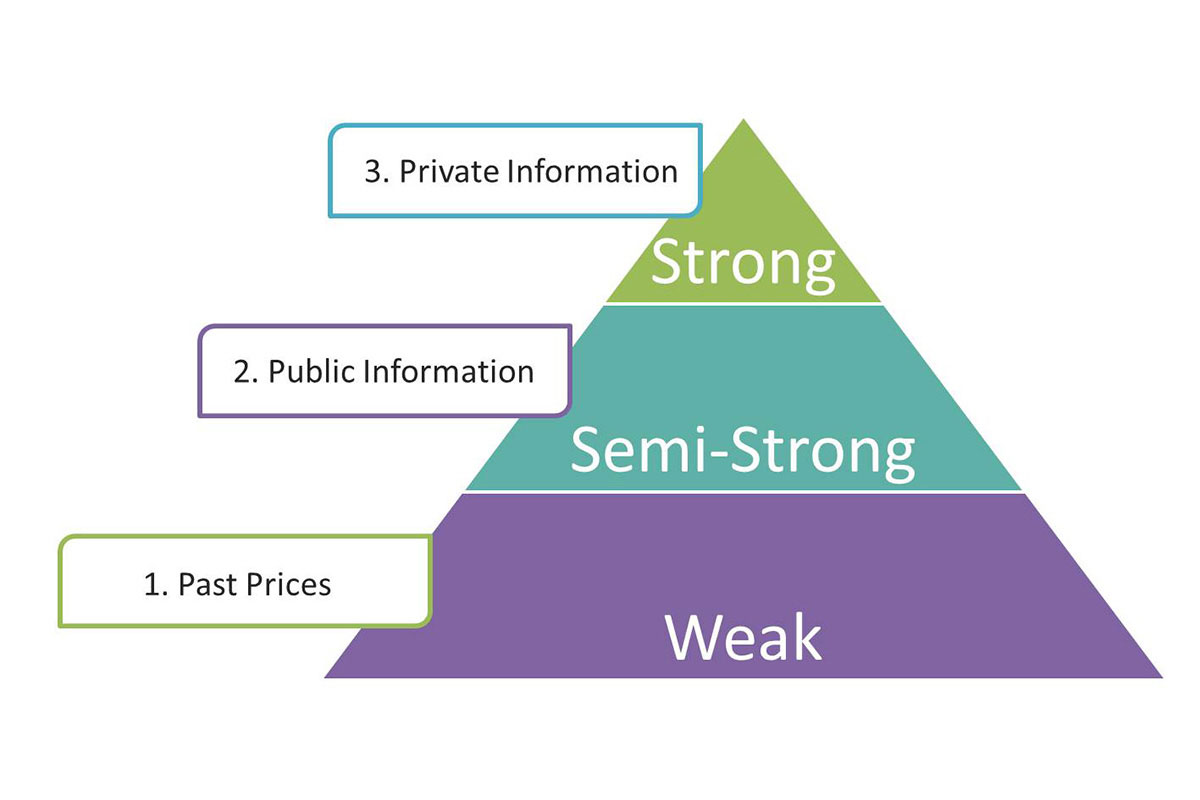
\includegraphics[width=13cm]{emh.jpg}
 				\caption{Os três níveis da HME, cada nível adiciona um tipo de informação cujo com o qual não seria possível prever um movimento de preço no mercado\cite{emh-article}.}
 				\label{fig:emh}
 			\end{figure}
 			\paragraph{}Não há uma reposta correta perante a validade da HME. Porém, muitos acadêmicos acreditam, pelo menos, na HME fraca\cite{emh-br}, fazendo com que, em algumas ocasiões, seja preferível a utilização da AF, ou seja, a análise de resultados financeiros, relatórios anuais e notícias divulgadas acerca do mercado financeiro.
 			
		\subsection{Índice de Bolsa de Valores}
			\paragraph{}Com objetivo de parametrizar algumas informações intrínsecas às bolsas, estas disponibilizam diversos índices. O principal índice da B3 é o Ibovespa, que é formado pelos ativos com maior volume negociado na bolsa nos últimos meses e indica, de forma resumida, o desempenho das ações negociadas na B3. Por ser um indicador principal, muitos fundos de investimento baseados no mercado de ações estão atrelados ao Ibovespa, contribuindo para a atratividade destes ativos de maneira geral.
			\begin{table}[h]
				\caption{Os 5 ativos com o maior volume e participação na B3, associados ao Ibovespa\cite{carteira-bovespa}.}
				\label{tab:courses}
				\centering
				{\footnotesize
					\begin{tabular}{|c|c|c|c|}
						\hline
						Código & Ação & Qtde. Teórica & Part.(\%)\\
						\hline
						ITUB4 &  Itaú Unibanco & 4.738.562.684 & 9,095 \\
						PETR4 &  Petrobras & 4.520.185.835 & 7,038 \\
						BBDC4 &  Bradesco & 3.873.597.664 & 7,028 \\
						VALE3 &  Vale S.A. & 3.147.743.563 & 8,414 \\
						ABEV3 &  AMBEV & 4.344.066.764 & 4,173 \\
						\hline
				\end{tabular}}
			\end{table}
			 
  \section{Aprendizado de Máquina}
  	\paragraph{}Pode-se definir Aprendizado de Máquina como o campo de estudo de algoritmos com o objetivo de fazer com que computadores possam agir sem serem explicitamente programados para fazer determinada tarefa. São algoritmos que analisam dados e aprendem com eles, para que assim possam fornecer uma predição de algo on mundo.
  	\paragraph{}Outra definição dada por Tom M. Mitchell\cite{ml-mitchell} fala que o campo de Aprendizado de Máquina busca responder a pergunta: ``Como podemos construir sistemas de computadores que possam automaticamente melhorar através de experiência e quais são as leis fundamentais que governam todo este processo de aprendizado?''. Outra definição do mesmo autor\cite{ml-mitchell-book} diz que ``Um programa de computador é dito aprender com a experiência E em respeito a uma tarefa T e medida pelo desempenho P se o seu desempenho em T, medido por P, melhora com a experiência E''. Neste conceito, se fosse desejado um programa de computador que aprendesse a classificar e-mails como spam ou não, por exemplo, poderíamos fazer a seguinte associação:
  	\begin{itemize}
  		\item E = A experiência de ver o usuário classificar emails como spam ou não.
			\item T = A tarefa de classificar os emails.
			\item P = O número ou fração de emails corretamente classificados como spam/não spam
  	\end{itemize}
  	\paragraph{}Geralmente, os algoritmos de Aprendizado de Máquina podem ser divididos em dois tipos: Aprendizado Supervisionado e Aprendizado Não Supervisionado.
  	\subsection{Aprendizado Supervisionado}
  		\paragraph{}Neste tipo, o algoritmo é inicialmente servido por uma série de dados rotulados cujo resultado já é conhecido. A ideia e que o algoritmo aprenda a criar uma estratégia para chegar ao resultado baseando-se nesses dados de modelo inicial. O aprendizado supervisionado pode ser dividido em problemas de regressão ou classificação.
  		\subsubsection{Problema de Regressão}
	  		\paragraph{}Neste tipo de problema, os dados de entrada (parâmetros) são mapeados em uma função contínua. Por exemplo, um algoritmo cujo objetivo fosse prever o preço dos imóveis na cidade do Rio de Janeiro baseando-se em dados como área útil, bairro, número de vagas na garagem, etc é considerado como um problema de regressão, pois o resultado final será um número contínuo, neste caso, o preço dos imóveis.
  		\subsubsection{Problema de Classificação}
  			\paragraph{}Neste caso, os parâmetros são mapeados de forma a classificar os dados em categorias distintas. Por exemplo, um algoritmo utilizado para prever se um tumor é benigno ou maligno a partir de dados como o tamanho, rugosidade do tumor e idade do paciente é considerado um problema de classificação, pois o resultado final será a categoria na qual o tumor pertence.
  			\paragraph{}TODO: falar sobre balanceamento
		\subsection{Aprendizado Não Supervisionado}
			\paragraph{}Neste tipo de aprendizado, não existe um conjunto inicial de dados e resultados, ou seja, nos permite abordar problemas onde temos pouca ou nenhuma ideia do que nossos resultados devem aparentar. Um exemplo, seria um algoritmo onde, utilizando uma coleção de 1000 artigos publicados por uma universidade, fizesse um agrupamento desses artigos, baseando-se em diferente variáveis como frequência de palavras semelhantes, número de paginas, etc.
		\subsection{Avaliação de Desempenho}
			\paragraph{}TODO: falar sobre as métricas utilizadas no pytext
  
  \section{Processamento de Linguagem Natural}
  	\paragraph{}Processamento de Linguagem Natural (PNL) se resume ao campo de estudo das tecnologias utilizadas para ajudar computadores a entenderem a linguagem natural dos humanos, é também considerado uma subárea da Inteligência Artificial. Pode ser usado em diversas aplicações\cite{simple-nlp}, como por exemplo:
  	\begin{itemize}
  		\item Aplicativos de tradução de idioma, como o Google Translator
  		\item Processamento de palavras, que empregam PNL para a correção gramática
  		\item Resposta de Voz iterativa em call centers, de forma a responder adequadamente conforme a requisição de usuários
  		\item Assistentes pessoais, como OK Google, Siri, Cortana e Alexa
  	\end{itemize}
	  \paragraph{}Geralmente, o PNL abrange um pré-processamento de texto antes deste ser transformado em uma forma inteligível por computadores, de forma a remover ruídos ou facilitar o processamento, e isto pode ocorrer de diversas formas.
	  \subsection{Sintaxe}
	  	\paragraph{}A sintaxe se refere à forma de como as palavras se organizam em uma sentença para que se obtenha sentido gramatical. Estas são algumas técnicas de sintaxe que podem ser utilizadas no pré-processamento de texto:
	  	\begin{itemize}
	  		\item Stemização: É a transformação de palavras flexionadas para sua forma radical. Por exemplo, as palavras ``estudos'', ``estudar'' e ``estudando'' se transformariam apenas em ``estud'', mas a palavra ``tiver" se transformaria em ``tiv'' e ``tenho" se transformaria em ``tenh''.
	  		\item Lematização: Semelhante à Stemização, porém, a palavra é resumida para seu lema, fazendo com que se alcance um nível maior de abstração. Neste caso, tanto a palavra ``tiver'' como ``tenho'' se transformaria no lema  ``ter''.
	  		\item Remoção de \textit{stopwords}: A remoção de ``palavras de parada'', ou seja, palavras como ``a'', ``de'', ``o'', ``da'', ``que'', ``e'', ``do'' é útil pois, na maioria das vezes, não são informações importantes para construção do modelo.
	  	\end{itemize}
  	\paragraph{}Além destas, outra técnicas mais simples são utilizadas, como a transformação de caracteres maiúsculos para minúsculos.
  	\subsection{Representação Vetorial}
  		\paragraph{}Após o pré-processamento, diversas técnicas podem ser utilizadas para a transformação do texto em números.. TODO
  		\subsubsection{\textit{Bag of Words}}
	  		\paragraph{}TODO
  		\subsubsection{Vetores Baseados em Redes Neurais}
  			\paragraph{}TODO
	  	
  \section{Redes Neurais}
  	\paragraph{}TODO
  	\subsection{Rede BilSTM Com Atenção}
	  	\paragraph{}TODO
  	\subsection{Rede CNN}
  		\paragraph{}TODO
  
  \section{PyText}
  	\paragraph{}TODO
  	\subsection{Configuração}
  		\paragraph{}TODO
  	\subsection{Uso}
  		\paragraph{}TODO
  
  \chapter{Obtenção e Pré-processamento de Dados}
  	\paragraph{}TODO
  	\section{Estratégia}
  		\paragraph{}TODO
  	\section{Pré-processamento}
  		\paragraph{}TODO
  
  \chapter{Treinamento}
	  \paragraph{}TODO
	  \section{Configuração}
		  \paragraph{}TODO
  	\section{Rotina de Treinamento}
  		\paragraph{}TODO
 		\section{Análise}
 			\paragraph{}TODO
  
  \chapter{Considerações Finais}
  	\paragraph{}TODO
  	\section{Conclusão}
  		\paragraph{}TODO
 		\section{Trabalhos Futuros}
 			\paragraph{}TODO

  \backmatter
  \bibliographystyle{coppe-unsrt}
  \bibliography{bibliography}

  \appendix

	\chapter{Rotinas e Arquivos de Configuração}
		\section{Rotina de Pré-processamento e Criação de Conjuntos de Dados}
		\section{Rotina de Criação de Arquivos de Configuração e Execução de Treinamentos}
		\section{Modelo de Arquivo de Configuração}

\end{document}
%% 
%%
%% End of file `example.tex'.
